%%%%%%%%%%%%%%%%%%%%%%%%%%%%%%%%%%%%%%%%%
% Simple Sectioned Essay Template
% LaTeX Template
%
% This template has been downloaded from:
% http://www.latextemplates.com
%
%
%%%%%%%%%%%%%%%%%%%%%%%%%%%%%%%%%%%%%%%%%

%----------------------------------------------------------------------------------------
%	PACKAGES AND OTHER DOCUMENT CONFIGURATIONS
%----------------------------------------------------------------------------------------

\documentclass[12pt]{article} % Default font size is 12pt, it can be changed here

\usepackage{geometry} % Required to change the page size to A4
\geometry{a4paper} % Set the page size to be A4 as opposed to the default US Letter

\usepackage{graphicx} % Required for including pictures

\usepackage{float} % Allows putting an [H] in \begin{figure} to specify the exact location of the figure
\usepackage{wrapfig} % Allows in-line images such as the example fish picture

\usepackage{lipsum} % Used for inserting dummy 'Lorem ipsum' text into the template

\linespread{1.2} % Line spacing

%\setlength\parindent{0pt} % Uncomment to remove all indentation from paragraphs

\graphicspath{{Pictures/}} % Specifies the directory where pictures are stored

\begin{document}

%----------------------------------------------------------------------------------------
%	TITLE PAGE
%----------------------------------------------------------------------------------------

\begin{titlepage}

\newcommand{\HRule}{\rule{\linewidth}{0.5mm}} % Defines a new command for the horizontal lines, change thickness here

\center % Center everything on the page

\textsc{\LARGE Politecnico di Milano}\\[1.5cm] % Name of your university/college
\textsc{\large Computer ethics}\\[0.5cm] % Minor heading such as course title

\HRule \\[0.4cm]
{ \huge \bfseries A case for bioprinting organs}\\[0.4cm] % Title of your document
\HRule \\[1.5cm]

\begin{minipage}{0.4\textwidth}
\begin{flushleft} \large
\emph{Author:}\\
Mirjam \textsc{Skarica} % Your name
\end{flushleft}
\end{minipage}
~
\begin{minipage}{0.4\textwidth}
\begin{flushright} \large
\emph{Supervisor:} \\
Prof.ssa Viola  \textsc{Schiaffonati} % Supervisor's Name
\end{flushright}
\end{minipage}\\[4cm]

{\large \today}\\[3cm] % Date, change the \today to a set date if you want to be precise

%\includegraphics{Logo}\\[1cm] % Include a department/university logo - this will require the graphicx package

\vfill % Fill the rest of the page with whitespace

\end{titlepage}

%----------------------------------------------------------------------------------------
%	TABLE OF CONTENTS
%----------------------------------------------------------------------------------------

\tableofcontents % Include a table of contents

\newpage % Begins the essay on a new page instead of on the same page as the table of contents 

%----------------------------------------------------------------------------------------
%	INTRODUCTION
%----------------------------------------------------------------------------------------

\section{Introduction} % Major section

Additive manufacturing, otherwise known as three-dimensional (3D) printing, is driving major innovations in many areas, such as engineering, manufacturing, art, education and medicine. Recent advances have enabled 3D printing of biocompatible materials, cells and supporting components into complex 3D functional living tissues. 3D bioprinting is being applied to regenerative medicine to address the need for tissues and organs suitable for transplantation. Compared with non-biological printing, 3D bioprinting involves additional complexities, such as the choice of materials, cell types, growth and differentiation factors, and technical challenges related to the sensitivities of living cells and the construction of tissues. Addressing these complexities requires the integration of technologies from the fields of engineering, biomaterials science, cell biology, physics and medicine. 3D bioprinting has already been used for the generation and transplantation of several tissues, including multilayered skin, bone, vascular grafts, tracheal splints, heart tissue and cartilaginous structures. Other applications include developing high-throughput 3D-bioprinted tissue models for research, drug discovery and toxicology.

Bioprinting is the three-dimensional printing of biological tissue and organs through the layering of living cells


Three dimensional (3D) printing is an additive manufacturing process. Meaning, it creates solid three-dimensional objects form a digital model by building up successive layers of material. It's one of the fastest growing fields and on top of it, it is the driving force behind innovations in many areas such as engineering, manufacturing and medicine. Ever since 3D printing of biomaterials has become possible, it has catalysed the field of bioprinting. Bioprinting creates a complex three dimensional functional and viable tissue by layering living cells onto a biologically compatible scaffolding. This is done with the intent of growing organs or structures to heal and promote growth in the body. 
 In this way numerous tissues cn constructed that can be used for a number of clinical applications from transplants to scientific research. 

http://www.forbes.com/sites/robertszczerba/2015/06/17/no-donor-required-5-body-parts-you-can-make-with-3-d-printers-2/
http://www.computerworld.com/article/2486998/emerging-technology/bio-printing-human-parts-will-spark-ethical--regulatory-debate.html?page=2
http://ethicsof3dprinting.weebly.com/bioprinting.html

%------------------------------------------------

\subsection{Subsection 1} % Sub-section

\lipsum[1] % Dummy text

%------------------------------------------------

\subsection{Subsection 2} % Sub-section

\lipsum[2] % Dummy text

%------------------------------------------------

\subsubsection{Subsubsection 1} % Sub-sub-section

\lipsum[3] % Dummy text

\begin{figure}[H] % Example image
\center{
\includegraphics[width=0.5\linewidth]{placeholder}}
\caption{Example image.}
\label{fig:speciation}
\end{figure}

%------------------------------------------------

\subsubsection{Subsubsection 2} % Sub-sub-section

\lipsum[4] % Dummy text

%----------------------------------------------------------------------------------------
%	MAJOR SECTION 1
%----------------------------------------------------------------------------------------

\section{Content Section} % Major section

\lipsum[5] % Dummy text

%------------------------------------------------

\subsection{Subsection 1} % Sub-section

\subsubsection{Subsubsection 1} % Sub-sub-section

\lipsum[6] % Dummy text

%------------------------------------------------

\subsubsection{Subsubsection 2} % Sub-sub-section

\lipsum[6] % Dummy text
\begin{wrapfigure}{l}{0.4\textwidth} % Inline image example
  \begin{center}
    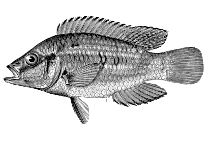
\includegraphics[width=0.38\textwidth]{fish}
  \end{center}
  \caption{Fish}
\end{wrapfigure}
\lipsum[7-8] % Dummy text

%------------------------------------------------

\subsubsection{Subsubsection 3} % Sub-sub-section

\begin{description} % Numbered list example

\item[First] \hfill \\
\lipsum[9] % Dummy text

\item[Second] \hfill \\
\lipsum[10] % Dummy text

\item[Third] \hfill \\
\lipsum[11] % Dummy text

\end{description} 

%----------------------------------------------------------------------------------------
%	MAJOR SECTION X - TEMPLATE - UNCOMMENT AND FILL IN
%----------------------------------------------------------------------------------------

%\section{Content Section}

%\subsection{Subsection 1} % Sub-section

% Content

%------------------------------------------------

%\subsection{Subsection 2} % Sub-section

% Content

%----------------------------------------------------------------------------------------
%	CONCLUSION
%----------------------------------------------------------------------------------------

\section{Conclusion} % Major section

\lipsum[12-13]

%----------------------------------------------------------------------------------------
%	BIBLIOGRAPHY
%----------------------------------------------------------------------------------------

\begin{thebibliography}{99} % Bibliography - this is intentionally simple in this template

\bibitem[Figueredo and Wolf, 2009]{Figueredo:2009dg}
Figueredo, A.~J. and Wolf, P. S.~A. (2009).
\newblock Assortative pairing and life history strategy - a cross-cultural
  study.
\newblock {\em Human Nature}, 20:317--330.
 
\end{thebibliography}

%----------------------------------------------------------------------------------------

\end{document}
